This another content chapter to tell the story of your research. 

\section{Introduction} \label{sec:intro}
The text can include anything you want. For example a citation using the \textit{$\backslash$cite} command \cite{icart_mini}. 


\subsection{More content}\label{sec:content}
You can also include some equations like Equation \ref{lowbound}. More info about equations and mathematical expressions: 
\href{https://www.overleaf.com/learn/latex/Mathematical_expressions}{Maths}.

\begin{equation}
    \label{lowbound}
    \underline{P}(x_q) = \min_{P(X_i|\pi_i) \in K(X_i|\pi_i)} \sum_{x_1,...,x_n \backslash x_q} \prod_{i=0}^n P(x_i|\pi_i)
\end{equation}

Include figures. More info on figures: \href{https://www.overleaf.com/learn/latex/Inserting_Images}{Figures}.

s
\begin{figure}[ht]
  \centering
  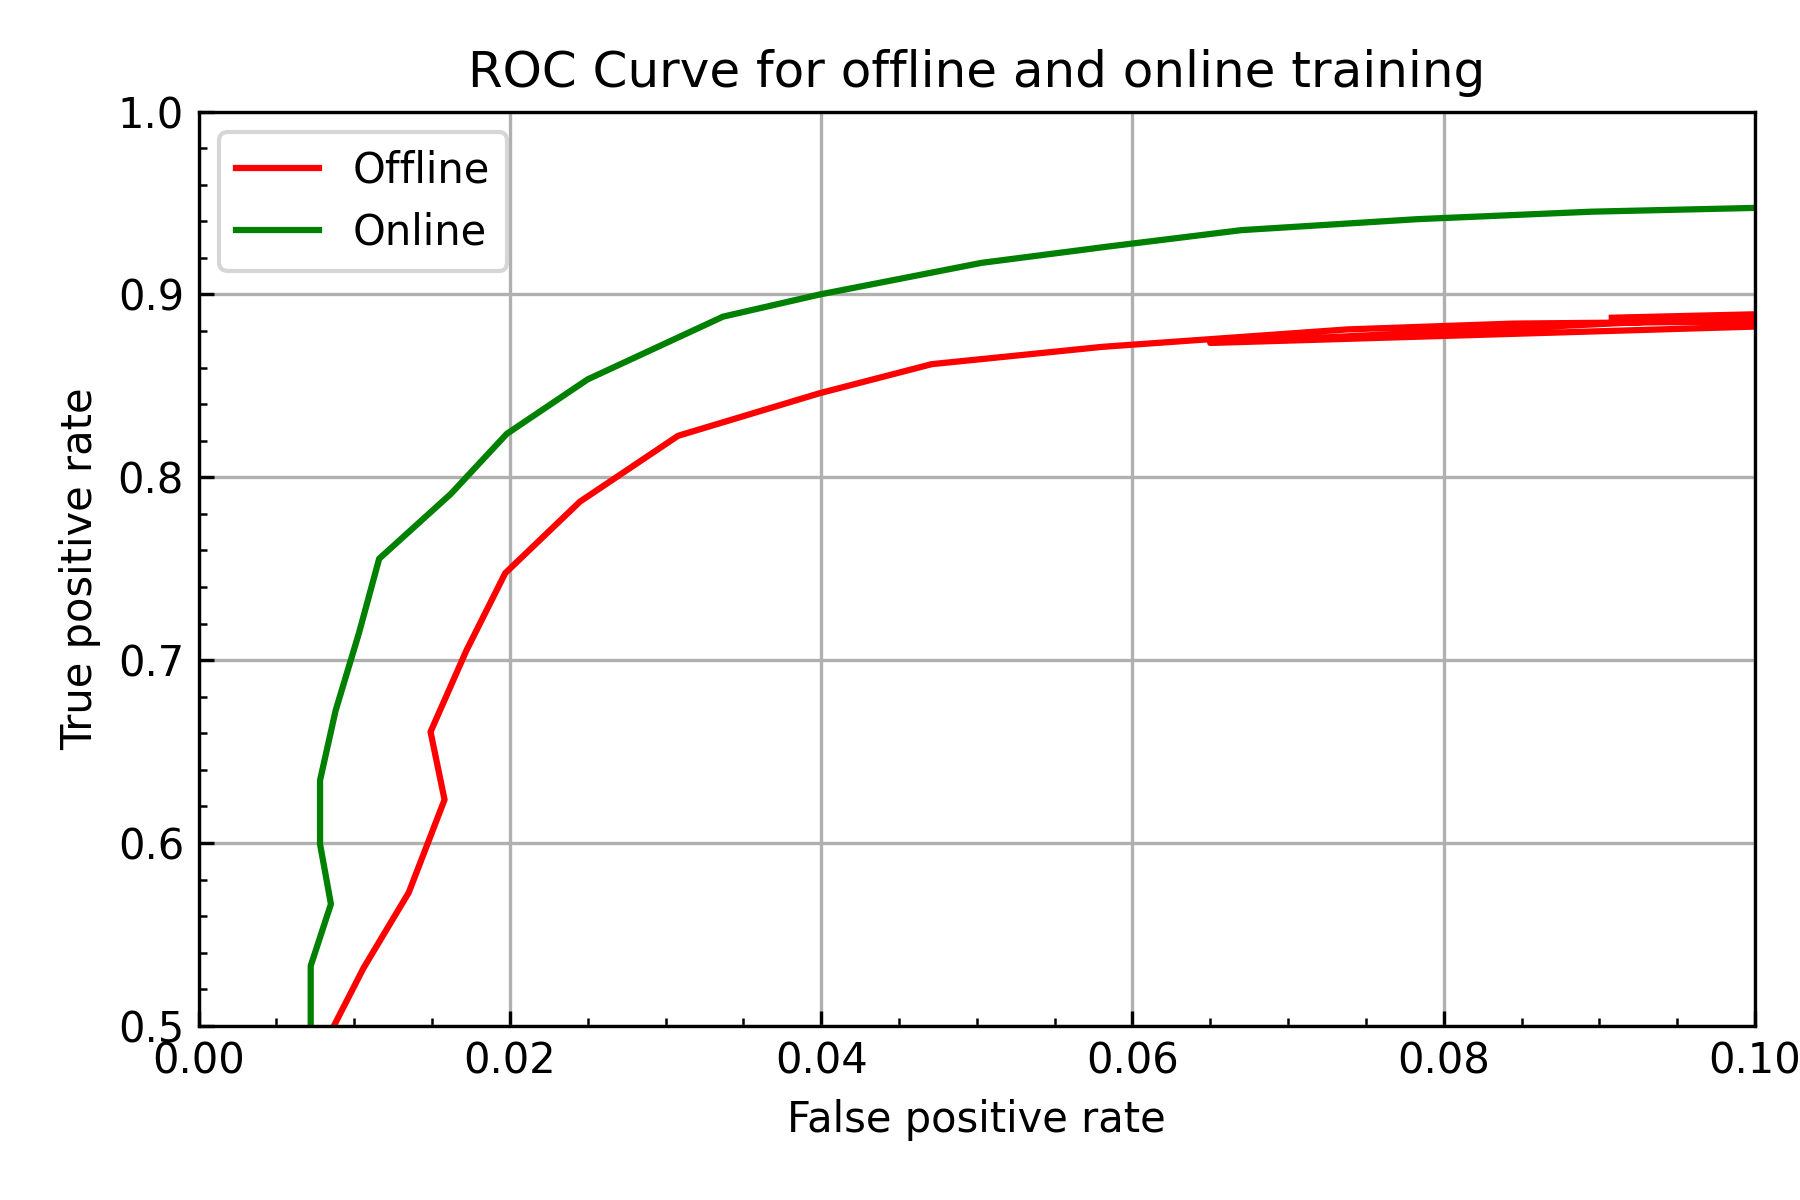
\includegraphics[scale=0.8]{figures/roc_offline.png}
  \caption{ROC Curve}
  \label{ROC Plot}
\end{figure} 

\begin{figure}[h]
    \centering
    % \hspace*{-8mm}
    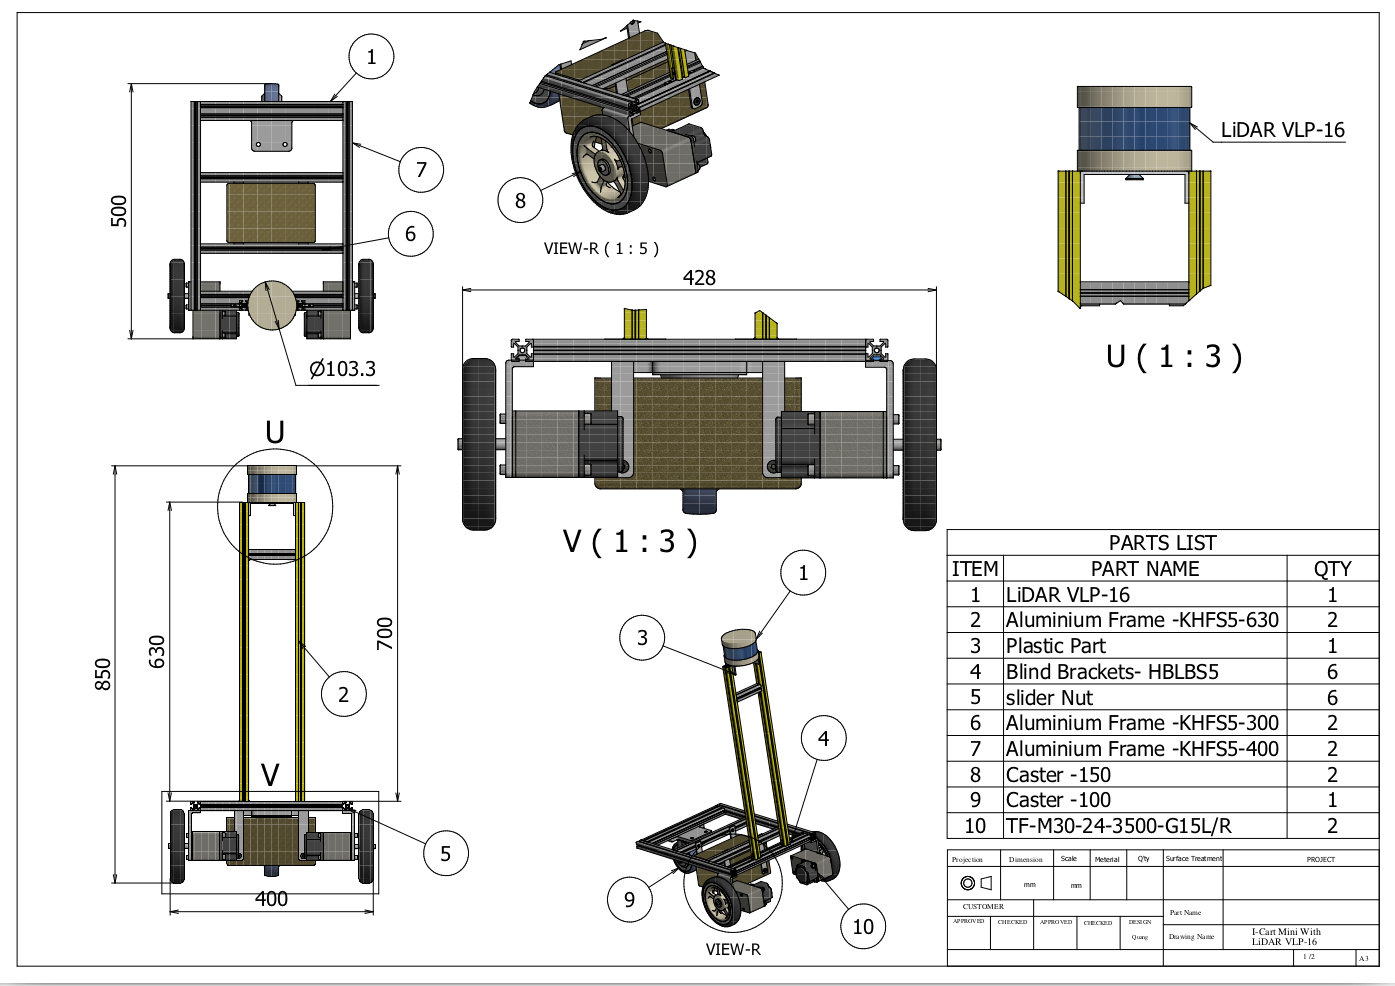
\includegraphics[width=1.0\linewidth]{Icart_mini_withLidar_drawing.png}
    \caption{Design drawing}
    \label{Fig1}
\end{figure}


Include Tables like Table \ref{tab:table}. More info on tables: 
\url{https://www.overleaf.com/learn/latex/Tables}.
\begin{table}[h]
    \centering
    \begin{tabular}{c|cc}
    \hline
    Disruption $\setminus$ $X^t$ & Available &  Unavailable \\ \hline \hline
    False      & $[0.952, 0.962]$ & $[0.038, 0.048]$ \\
    True       & $[0.038, 0.048]$ & $[0.952, 0.962]$ \\ \hline
    \end{tabular}
    \caption{This is a table} 
    \label{tab:table}
\end{table}



